\chapter{Variational Principles and Lagrange's Equations}
\section{Hamilton's Principle}
\subsection{Configuration Space}
\begin{itemize}
	\item The Instantaneous configuration of a system is described by the values of $n$ generalized coordinates $q_1,    q_n$ and corresponds to a particular point in a cartesian hyperspace where the q's from the $n$  diamensional space is known as configuration space.
	\item As time goes by, the state of the system changes and the system point moves in configuration space tracing out a curve, described as "the path of motion of the system".
	\item The motion of the system then refered to the motion of the system point along this path in configuration space
	\item Time can be considered formally as a parameter of the curve to each point on the path there is associated one or more values of the time. Each point on the path represent the entire system  configuration at some given instant of time.\\\\
	\textbf{Monogenic System}: The mechanical systems whose motion for which all forces  (except the forces of constraint) are derivable from a generalized scalar potential that may be a function of the coordinates, velocities and time.
\end{itemize}
	\subsection{Hamilton's Principle}
	The motion of the system from time $t_1 $ to time $t_2$ is such that the line integral called the avtion or the action integral.
	\begin{equation}
	I=\int\limits_{t_1}^{t_2}Ldt
	\end{equation}
	where $L$ is $T-V$ has stationary value for the actual path of the motion.\\\\
	ie. out of all possible path by which the system point could travel from it's position at time $t_1$ to its position at time $t_2$. It will travel along that path for which the value of integral is stationary.\\\\
	$\therefore$ Hamilton's principle can summarize by saying that the motion is such that the variation of the line integral $I$ for fixed $t_1$ and $t_2$ is zero.
	\begin{equation}
		\delta I=\delta\int\limits_{t_1}^{t_2}L(q_1,.....q_n,\dot{q}_1.....\dot{q}_n,t)dt=0
	\end{equation}
	Where the system constraints are holonomic, Hamilton's principle is both a necessary and suffitient condition for lagrange's equations.
	\section{Calculus of Variation}
	Consider a one diamensional problem, we have a function $f(y,\dot{y},x)$ defined on a path $y-y(x)$  between two value $x_1$ and $x_2$ where $\dot{y}$ is the derivative of $y$ with respect to $x$.\\\\
	To find a particular path y(x) such that the line integral $y$ of the function $f$ between $x_1$ and $x_2$\\
	$ \dot{y}\equiv \frac{dy}{dx}$
	\begin{equation}
	J=\int\limits_{x_1}^{x_2}f(y,\dot{y},x)dx
	\end{equation}
 	has stationary value relative to paths differing infinitesimally from the correct function $y(x)$.\\\\
 	Since $J$ must have a stationary value for the correct path relative to any neighboring path, the variation must be zero relative to some particular set of neighboring paths labeled by an infinitesimal parameter $\alpha$.\\
 	such a set of varied path given by 
 	\begin{equation}
 	y(x,\alpha)=y(x,0)+\alpha \eta(x)\label{VP-eq04}
 	\end{equation}
	$y(x,0)$- Correct path\\
	$\eta(x)$-any function vanishes at $x=x_1$ and $x=x_2$\\\\
	Assume both the correct path $y(x)$ and the auxillary function $\eta(x)$ are well behaved functions between $x_1$ and $x_2$. For such any parametric family of curves, $J$ is also a function of $\alpha$
	\begin{equation}
	J(\alpha)=\int\limits_{x_1}^{x_2}f(y(x,\alpha),\dot{y}(x,\alpha),x)dx
	\end{equation}
	 Condition for obtaining stationary points is 
	 \begin{equation}
	 \left( \frac{dJ}{d\alpha}\right) _{\alpha=0}=0
	 \end{equation}
	differentiating under integral sign 
	\begin{equation}
	\frac{d J}{d \alpha}=\int_{x_{1}}^{x_{2}}\left(\frac{\partial f}{\partial y} \frac{\partial y}{\partial \alpha}+\frac{\partial f}{\partial \dot{y}} \frac{\partial \dot{y}}{\partial \alpha}\right) d x
	\end{equation}
	For the second term, integrating by parts\\
	\begin{align*}
		\int_{x_{1}}^{x_{2}} \frac{\partial f}{\partial \dot{y}} \frac{\partial \dot{y}}{\partial \alpha} d x&=\int_{x_{1}}^{x_{2}} \frac{\partial f}{\partial \dot{y}} \frac{\partial^{2} y}{\partial x \partial \alpha} d x\\
		&=\left.\frac{\partial f}{\partial \dot{y}} \frac{\partial y}{\partial \alpha}\right|_{x_{1}} ^{x_{2}}-\int_{x_{1}}^{x_{2}} \frac{d}{d x}\left(\frac{\partial f}{\partial \dot{y}}\right) \frac{\partial y}{\partial \alpha} d x
	\end{align*}
All the varied curves pass through $(x_1,y_1),(x_1,y_1)$ and hence the partial derivative of $y$ with respect to  $\alpha$ $x_1$ and $x_2$ must vanish.
\begin{equation}
\therefore \frac{d J}{d \alpha}=\int_{x_{1}}^{x_{2}}\left(\frac{\partial f}{\partial y}-\frac{d}{d x} \frac{\partial f}{\partial \dot{y}}\right) \frac{\partial y}{\partial \alpha} d x
\end{equation}
Therefore, the condition for stationary value
\begin{equation}
\left(\frac{dJ}{d\alpha} \right)_{\alpha=0} =\int_{x_{1}}^{x_{2}}\left(\frac{\partial f}{\partial y}-\frac{d}{d x} \frac{\partial f}{\partial \dot{y}}\right) \frac{\partial y}{\partial \alpha} d x=0\label{VP-eq09}
\end{equation}
Where $\left( \frac{\partial y}{\partial \alpha}\right) $ is a function of $x$ that is arbitrary except for continuity and end point conditions.
\begin{itemize}
	\item \textit{Fundemental lemma} of calculus of variation
	\begin{equation}
	\text{if} \int\limits_{x_1}^{x_2}M(x)\eta(x)dx=0
	\end{equation}
	\textit{For all arbitrary functions $\eta (x)$ continuous through the second derivative, then $M(x)$ must identically vanish in the interval $(x_1,x_2)$}
\end{itemize}
	For a particular parametric family of varied paths given by \ref{VP-eq04}
	$$\left(\frac{\partial y}{\partial\alpha} \right)_0 =\eta(x)\text{the arbitrary function}$$
	$\therefore$ from \ref{VP-eq09} using fundamental lemma, we get 
	\begin{equation}
	\frac{\partial f}{dy}-\frac{d}{dx}\left( \frac{\partial f}{\partial\dot{y}}\right) =0\label{VP-11}
	\end{equation}
	\begin{itemize}
		\item The infinitesimal departure of the varied path from the correct path $y(x)$ at the point $x$ and thus corresponds to virtual displacement $\delta y$ is
		$$\left( \frac{\partial y}{\partial\alpha}\right)_0 d\alpha=\delta y$$
\item Similarly, infinitesimal variation of $y$ above the correct path is given as		
		$$\left( \frac{\partial y}{\partial\alpha}\right)_0 d\alpha=\delta J$$
		$$\delta J=\int_{x_{1}}^{12}\left(\frac{\partial f}{\partial y}-\frac{d}{d x} \frac{\partial f}{\partial \dot{y}}\right)\delta y\ dx=0$$
	\end{itemize}
\textbf{Euler-Lagrange Differential Equation}\\
Let $f$ is a function of many independent variables $y_i$, and their relatives $\dot{y}_i$. Where $y_i$ and $\dot{y}_i$ are functions of parametric variable $x$.
\begin{equation}
\delta J=\delta \int_{1}^{2} f\left(y_{1}(x) ; y_{2}(x), \ldots, \dot{y}_{1}(x) ; \dot{y}_{2}(x), \cdots, x\right)_{d_{x}}\label{VP-12}
\end{equation}
\begin{align*}
y_{1}(x, \alpha)&=y_{1}(x, 0)+\alpha \eta_{1}(x),\\
y_{2}(x, \alpha)&=y_{2}(x, 0)+\alpha \eta_{2}(x)\\
\vdots\quad&\hspace{1cm}\vdots\hspace{1.2cm}\vdots
\end{align*}
By using fundamental lemma, the condition that $\delta J$ is zero requires coeffitient of $\delta y_i$ seperately vanish
\begin{equation}
\frac{\partial f}{\partial y_{i}}-\frac{d}{d x} \frac{\partial f}{\partial \dot{y}_{i}}=0\label{VP-13}
\end{equation}
This is the appropriate generalization of equation \ref{VP-11} to several variables and known as the Euler-Lagrange differential equation.\\\\
\textbf{Langrange's Equation}\\
For the integral in Hamilton principle
$$I=\int_{1}^{2} L\left(q_{i}, \dot{q}_{i}, t\right) d t$$
have same form as equation \ref{VP-12}, with transformation 
$$x\rightarrow t$$
$$y_i\rightarrow q_i$$
$$f(y_i,\dot{y}_i,x)\rightarrow L(q_i,\dot{q}_i,t)$$
as we assumed $y_i$ variables are independent the corresponding $q_i$ generalized coordinates are independent which requires that the constraints be holonomic.\\
The Euler-Lagrange equation corresponding to the integral $I$ then become the Lagrange equations of motion 
$$\frac{d}{d t} \frac{\partial L}{\partial \dot{q}_{i}}-\frac{\partial L}{\partial q_{i}}=0$$
Lagrange's equations follow Hamilton's principle for monogenic systems with holonomic constraints \\\\
\textbf{Lagrange Undetermined Multipliers}\\
used to solve systems with holonomic constraints as well as certain types of non-holonomic systems. \\
If there are $n$ variables and $m$ constraint equations $f\alpha$ of the form
$$f(r_1,r_2,r_3....t)=0$$
the extra virtual displacements are eliminated by the method of Lagrange undetermined multipliers.
$$I=\int_{1}^{2}\left(L+\sum_{\alpha=1}^{m} \lambda_{\alpha} f_{a}\right) d t$$
allow the $q_2$ and the $\lambda_\alpha$ to be vary independently to obtain $n+m$ equations.\\
variations of $\lambda_\alpha$ gives the $m$ constraint equations the variations of the $q-i$'s give
$$\delta I=\int_{1}^{2} d t\left(\sum_{i=1}^{n}\left(\frac{d}{d t} \frac{\partial L}{\partial \dot{q}_{i}}-\frac{\partial L}{\partial q_{i}}+\sum_{\alpha=1}^{m} \lambda_{a} \frac{\partial f_{a}}{\partial q_{i}}\right) \delta q_{i}\right)=0$$
The $\delta q_i$'s are not independent we choose the $\lambda_{\alpha}$'s so that $m$ of the $n$ equations are satisfied for arbitrary $\delta q_i$, and then choose variations of the $\delta q_i$ in the remaining $n-m$ equations independently.\\
Thus we obtain $m$ equations of the form
$$\frac{d}{d t} \frac{\partial L}{\partial \dot{q}_{k}}-\frac{\partial L}{\partial q_{k}}+\sum_{\alpha=1}^{m} \lambda_{a} \frac{\partial f_{a}}{\partial q_{k}}=0$$
$Q_k$ are generalized forces\\
$Q_k$ have the magnitute of the forces needed to produce the individual constraints.\\\\
\section{Generalized Momentum}
If $L$ is the Lagrangian of a system then the generalized momentum associated with the coordinate $q_j$ shall be defined as
$$P_j=\frac{\partial L}{\partial \dot{q}_j}$$
The terms canonical momentum and conjugate momentum are often also used for $P_j$\\
If $q_j$ is not cartisian coordinate $P_j$ does not necessarilu have the diamensios of a linear momentum. If there is a velocity dependent potential then even with a cartesian coordinate $q_j$ the associated generalized momentum will not be indentical with mechanical momentum.
\section{Cyclic coordinate and Generalized Momentum Conjugate }
If the Lagrangian of a system does not contain a given generalized coordinate $q_j$ explicitly (although it may contain the corresponding velocity $\dot{q}_j$ ) then the coordinate is said to be cyclic or ignorable.
\begin{align*}
\intertext{The Lagrange equation of motion}
\frac{d}{dt}\left( \frac{\partial L}{\partial \dot{q}_j}\right)-\frac{\partial L}{\partial q_j} &=0
\intertext{reduces for cyclic coordinate, to}
\frac{d}{dt}\left(\frac{\partial L}{\partial \dot{q}_j} \right) &=0
\intertext{or}
\frac{dP_j}{dt}&=0
\intertext{Which means}
P_j&=\text{constant}
\therefore& \text{The generalized momentum conjugate to a cyclic coordinate is conserved}
\end{align*}
\begin{itemize}
	\item This general rule for cyclic coordinates contain all the conservation theorems discussed before 
	\item With proper restriction it should reduces to the conservation theorems. 
	\item The consevation theorems ate closely related to the symmetry properties of the system.
\end{itemize}
\begin{note}
	If any system or any function representing a property of the system does not change under some operation carried on the system, the system is said to possess symmetry with respect to that operation 
\end{note}
\section{Conservation of Linear Momentum}
Consider a generalized coordinate $q_j$ for which $dq_j$ represents a translation of the system as a swhole in some given direction.
\begin{align*}
\intertext{Then $q_j$ cannot appear in $T$ for velocities are not affected by a shift in the origin}
\therefore \frac{\partial T}{\partial q_j}=0
\intertext{assume a consevative system for which $V$ is not function of the velocities}
\therefore \text{Lagrange's equation of motion}\\
\frac{d}{dt}\left(\frac{\partial  T}{\partial \dot{q}_j} \right) \equiv\dot{P}_j=\frac{-\partial V}{\partial q_j}=Q_j
\intertext{Where $Q_j$ is the component of the total force along the direction of translation of $q_j$ and $P_j$ is the component of total linear momentum.}
\text{if}q_j\text{ is cyclic, then}\\
\frac{-\partial V}{\partial q_j}\equiv Q_j=0
\end{align*}
ie. conservation theorem if a geven component of the total applied force vanishes, the corresponding component of the linear momentum is conserved\\
\textit{If the system is invarient under translation along a given direction (homogeneily of space) the corresponding linear momentum is conserved}\\
Then the physical properties of a closed system are not affected by an arbitrary displacement\\\\
\section{Conservation of Angular Momentum}
If a cyclic coordinate $q_j$ is such that $dq_j$ corresponds to a rotation of the system of particles around some axis, then the consevation of it's conjugate momentum corresponds to consetvation of angular momentum.\\
$T$ cannot cantain $q_j$ for a rotation of the coordinate system cannot affect the magnitude of velocities.
$$\therefore \frac{\partial T}{\partial q_j}=0$$
$V$ is independent of $\dot{q}_j$ as before\\
If the rotation coordinate $q_j$ is cyclic then $Q_j$, which is the component of applied torque along $\hat{n}$ vanishes and the component of $L$ along $n$ is constant. ie angular momentum conservation.\\
\textit{If the generalized rotation coordinate is cyclic, (and conjugate angular momentum is conserved) the system is invarient under rotation (homogeneily of angle) ie properties of closed system will not change due to arbitrary rotation about the origin of the frame of reference.}
\begin{exercise}
	 A particle of mass $m$ moves inside a bowl under gravity. If the surface of the bowl is given by the equation $z=\frac{1}{2} a\left(x^{2}+y^{2}\right)$, where $a$ is a constant.\\
	(a) Write down Lagrangian of the system in cylindrical coordinate.\\
	(b) Identify the cyclic coordinate and law of conservation of momentum.\\
	(c) Write down the equation of motion
\end{exercise}	
\begin{answer}
	\begin{align*}
	\text{There is only one particle, so }N&=1\\
	\text{Cartesian coordinate kinetic energy is }T&=\frac{1}{2} m\left(\dot{x}^{2}+\dot{y}^{2}+\dot{z}^{2}\right)\text{ and potential energy is} V=m g z
	\intertext{Equation of Constraint is -}
	\intertext{1. Particle is constrained to move on surface of a bowl, so the equation of constraint is}
	z&=\frac{1}{2} a\left(x^{2}+y^{2}\right) \text {, so } k=1\\
	\text{Degree of freedom }( DOF) &=3 N-k=3 \times 1-1=2
	\intertext{Hence, there are two degree of freedom, so we need two generalized coordinates.}
	\intertext{Now transforming the Cartesian coordinate to cylindrical coordinate, $x=r \cos \theta, y=r \sin \theta$, z=z}
	\intertext{So, the kinetic energy is $T=\frac{1}{2} m\left(\dot{r}^{2}+r^{2} \dot{\theta}^{2}+\dot{z}^{2}\right)$. And the equation of constraint in cylindrical coordinate $\left(z=\frac{1}{2} a r^{2}\right)$ is written as $\dot{z}=a r \dot{r}$}
	\intertext{So, kinetic energy for two degree of freedom with suitable coordinate is given by, $T=\frac{m}{2}\left(\dot{r}^{2}+r^{2} \dot{\theta}^{2}+a^{2} r^{2} \dot{r}^{2}\right)$ and potential energy $V=\frac{m g a r^{2}}{2}$}
	T=\frac{m}{2}\left(\dot{r}^{2}+r^{2} \dot{\theta}^{2}+a^{2} r^{2} \dot{r}^{2}\right)&\text{ and potential energy }V=\frac{m g a r^{2}}{2}\\
	\text{So, Lagrangian is }L&=\frac{m}{2}\left[\dot{r}^{2}\left(1+a^{2} r^{2}\right)+r^{2} \dot{\theta}^{2}-a g r^{2}\right]
	\intertext{(b) Hence, $\frac{\partial L}{\partial \theta}=0$ so, $\theta$ is cyclic coordinate hence $p_{\theta}=\frac{\partial L}{\partial \dot{\theta}}=m r^{2} \dot{\theta}$ is a constant of motion, which is identified as angular momentum of the system. So angular momentum of the system is conserved.}
\text{	(c) If Lagrangian of the system is } L&=\frac{m}{2}\left[\dot{r}^{2}\left(1+a^{2} r^{2}\right)+r^{2} \dot{\theta}^{2}-a g r^{2}\right]\text{ then}\\
\text{Equation of Motion is }&\frac{d}{d t}\left(\frac{\partial L}{\partial \dot{r}}\right)-\frac{\partial L}{\partial r}=0\\
\left(\frac{\partial L}{\partial r}\right)&=m \dot{r}^{2} a^{2} r+m r \dot{\theta}^{2}-m a g r\text{ and }\left(\frac{\partial L}{\partial \dot{r}}\right)=m \dot{r}\left(1+a^{2} r^{2}\right)\\
\Rightarrow \frac{d}{d t}\left(\frac{\partial L}{\partial \dot{r}}\right)&=m \ddot{r}\left(1+a^{2} r^{2}\right)+m \dot{r} a^{2} 2 r \dot{r}=m \ddot{r}\left(1+a^{2} r^{2}\right)+2 m a^{2} r \dot{r}^{2}\\
\frac{d}{d t}\left(\frac{\partial L}{\partial \dot{r}}\right)-\frac{\partial L}{\partial r}&=0 \Rightarrow m \ddot{r}\left(1+a^{2} r^{2}\right)+2 m a^{2} r \dot{r}^{2}-m a^{2} r \dot{r}^{2}-m r \dot{\theta}^{2}+m a g r=0\\
\Rightarrow m \ddot{r}\left(1+a^{2} r^{2}\right)&+m a^{2} r^{2}-m r \dot{\theta}^{2}+m a g r=0
	\end{align*}
\end{answer}
\begin{exercise}
 A mass $m$ is attached to one end of spring with spring constant $k$ and natural length $l$. The other end is pivoted at point $O$ as shown in figure. If the particle is constrained to move in $x-y$ plane under gravity (in $y$ direction)\\
 (a) Write down the expression for kinetic energy and potential energy.\\
 (b) Write down Lagarngian in Cartesian coordinate system.\\
 (c) Transform the Lagrangian in suitable coordinate system.\\
 \begin{figure}[H]
 	\centering
 	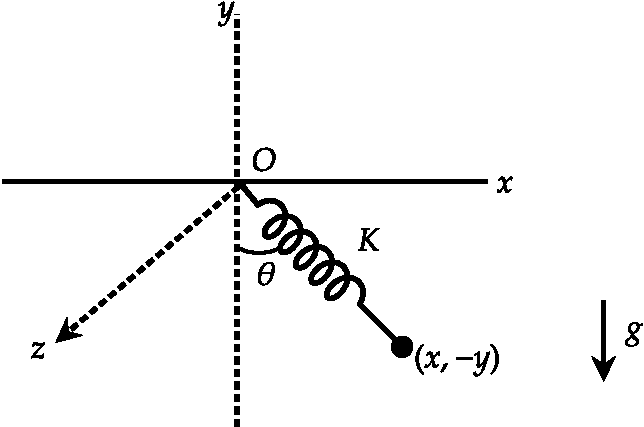
\includegraphics[height=3.8cm,width=5.5cm]{VP-01}
 \end{figure}
\end{exercise}
\begin{answer}
	\begin{align*}
	\intertext{ (a) Number of particle $N=1$, kinetic energy is given by $T=\frac{1}{2} m\left(\dot{x}^{2}+\dot{y}^{2}+\dot{z}^{2}\right)$, potential energy is given by $V=-m g y .$}
	\intertext{Equation of Constraint is -}
	\text{The particle is constrained to move in }&x-y\text{ plane so equation of constraint }z=0 \Rightarrow k=1\\
	\text{So, degree of freedom }( \text{ DOF } )&=3 N-K=3 \times 1-1=2
	\intertext{If degree of freedom is two then there must be two independent motion.}
	z&=0 \Rightarrow \dot{z}=0
	\intertext{So, $T=\frac{1}{2} m\left(\dot{x}^{2}+\dot{y}^{2}\right)$ and $V=-m g y+\frac{1}{2} k\left[\sqrt{\left(x^{2}+y^{2}\right)}-l\right]^{2}$ (potential energy due to gravity and stored energy due to spring).}
	\intertext{Lagrangian in the Cartesian coordinate is $L=\frac{1}{2} m\left(\dot{x}^{2}+\dot{y}^{2}\right)-\left(-m g y+\frac{1}{2} k\left[\sqrt{\left(x^{2}+y^{2}\right)}-l\right]^{2}\right)$,
		$$
		L=\frac{1}{2} m\left(\dot{x}^{2}+\dot{y}^{2}\right)+m g y-\frac{1}{2} k\left[\sqrt{\left(x^{2}+y^{2}\right)}-l\right]^{2}
		$$}
	\end{align*}
	(b) These two independent motions are in (i) radial direction and (ii) angular direction in plane so best coordinate system to define the system is circular polar coordinate.\\
	But one should express the Lagrangian into suitable coordinate which must be independent of radial and angular variable.
	\begin{align*}
	\text{Put }x&=r \sin \theta, y=r \cos \theta,\text{ so, Lagrangian is given by -}\\
	L&=\frac{1}{2} m\left(\dot{r}^{2}+r^{2} \dot{\theta}^{2}\right)+m g r \cos \theta-\frac{1}{2} k(r-l)^{2}\\
	\text{The equation of }&\text{motion in terms of variable $r$ is }\frac{d}{d t}\left(\frac{\partial L}{\partial \dot{r}}\right)-\frac{\partial L}{\partial r}=0\\
	&\left(\frac{\partial L}{\partial \dot{r}}\right)=m \dot{r} \Rightarrow \frac{d}{d t}\left(\frac{\partial L}{\partial \dot{r}}\right)=m \ddot{r} \text { and }\left(\frac{\partial L}{\partial r}\right)=m r \dot{\theta}^{2}+m g \cos \theta-k(r-l) \\
	&\frac{d}{d t}\left(\frac{\partial L}{\partial \dot{r}}\right)-\frac{\partial L}{\partial r}=0 \Rightarrow m \ddot{r}-m r \dot{\theta}^{2}-m g \cos \theta+k(r-l)=0
	\intertext{The equation of motion in terms of variable $\theta$}
	\left(\frac{\partial L}{\partial \dot{\theta}}\right)&=m r^{2} \dot{\theta}\left(\frac{\partial L}{\partial \theta}\right)=-m g r \sin \theta\\
	\frac{d}{d t}\left(\frac{\partial L}{\partial \dot{\theta}}\right)&=m r^{2} \ddot{\theta}+2 m r \dot{r} \dot{\theta}\\
	\frac{d}{d t}\left(\frac{\partial L}{\partial \dot{\theta}}\right)-\frac{\partial L}{\partial \theta}&=0 \Rightarrow m r^{2} \ddot{\theta}+2 m r \dot{r} \dot{\theta}+m g r \sin \theta=0
	\end{align*}
\end{answer}
\begin{exercise}
	 A spherical pendulum of length $a$ moves in a space about fixed point $O$.\\
	(a) Write down Lagrangian of the system.\\
	(b) Identify cyclic Coordinate\\
	(c) Solve Lagrangian equation of motion.\\
	\begin{figure}[H]
		\centering
		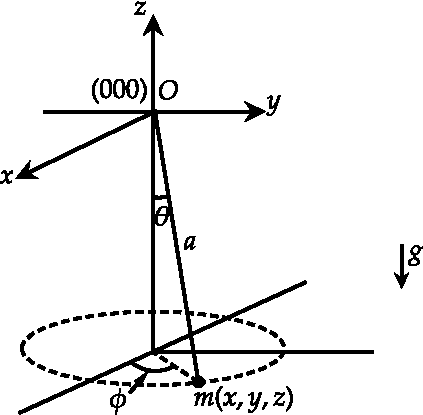
\includegraphics[height=5cm,width=6cm]{VP-02}
	\end{figure}
\end{exercise}
\begin{answer}
	\begin{align*}
	\text{Number of particle }N&=1\text{ so }T=\frac{1}{2} m\left(\dot{x}^{2}+\dot{y}^{2}+\dot{z}^{2}\right)\text{ and potential}\\
	\text{energy of system is }V&=-m g z
	\intertext{Equation of Constraint is -}
	\text{(1) The length of pendulum is fixed }&\sqrt{x^{2}+y^{2}+z^{2}}=a\text{ so }K=1\\
	\text{So, degree of freedom }&(\mathrm{DOF})=3 . N-K=3.1-1=2
	\intertext{So there is a need of two generalized coordinates to solve the equation of motion. There are two independent motion (i) angular motion of particle from $z$-axis (ii) angular motion in $x-y$ plane about $z$ axis.}
	\intertext{So, suitable coordinate is spherical coordinate.}
	x&=r \sin \theta \cos \phi, y=r \sin \theta \sin \phi, z=r \cos \theta\\
\text{	From equation }&\text{of constraint, }r=a \Rightarrow \dot{r}=0\\
\text{Kinetic energy }T&=\frac{1}{2} m\left(a^{2} \dot{\theta}^{2}+a^{2} \sin ^{2} \theta \dot{\phi}^{2}\right), \text{potential energy }V=-m g a \cos \theta\\
L=T-V&=\frac{1}{2} m\left(a^{2} \dot{\theta}^{2}+a^{2} \sin ^{2} \theta \dot{\phi}^{2}\right)+m g a \cos \theta\\
\text{(b) }\frac{\partial L}{\partial \phi}=0\text{ so }\phi\text{ is cyclic coordinate }\frac{\partial L}{\partial \dot{\phi}}&=p_{\phi}=m a^{2} \sin ^{2} \theta \dot{\phi}\text{ is constant of motion.}\\
\text{(c) }\frac{d}{d t}\left(\frac{\partial L}{\partial \dot{\theta}}\right)-\left(\frac{\partial L}{\partial \theta}\right)&=0\\
\left(\frac{\partial L}{\partial \dot{\theta}}\right)=m a^{2} \dot{\theta} \Rightarrow \frac{d}{d t}\left(\frac{\partial L}{\partial \dot{\theta}}\right)&=m a^{2} \ddot{\theta} \Rightarrow\left(\frac{\partial L}{\partial \theta}\right)=m a^{2} \sin \theta \cos \theta \dot{\phi}^{2}-m g a \sin \theta\\
\text{So, }\frac{d}{d t}\left(\frac{\partial L}{\partial \dot{\theta}}\right)-\left(\frac{\partial L}{\partial \theta}\right)&=0 \Rightarrow m a^{2} \ddot{\theta}-m a^{2} \sin \theta \cos \theta \dot{\phi}^{2}+m g a \sin \theta=0
	\end{align*}
\end{answer}
\begin{exercise}
	 A particle of mass $m$ is constrained to move under gravity in inner surface of cone of half angle $\alpha$ as shown in figure.\\
	(a) Write down Lagrangian in suitable coordinate system\\
	(b) Identify cyclic coordinate and discuss conservation of momentum\\
	(c) Write down Lagrange's equation of motion\\
	\begin{figure}[H]
		\centering
		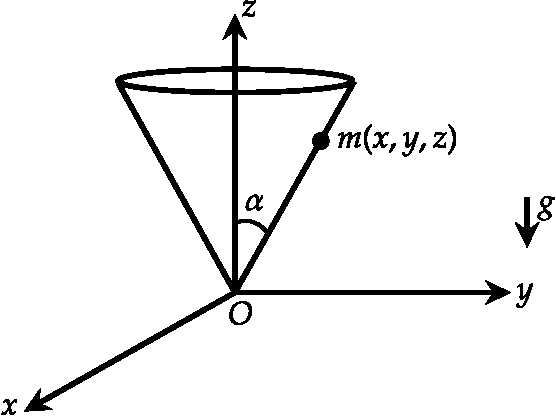
\includegraphics[height=3.5cm,width=5cm]{VP-03}
	\end{figure}
\end{exercise}
\begin{answer}$\left. \right. $\\
	\begin{figure}[H]
		\centering
		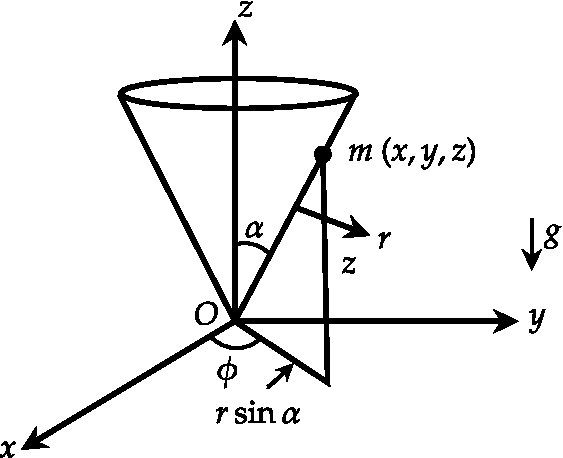
\includegraphics[height=4cm,width=5cm]{VP-04}
	\end{figure}
	\begin{align*}
	\intertext{ A particle of mass $m$ is constrained to move in inner surface of cone of half angle $\alpha$ and $x, y, z$ are the coordinates of particle at any time $t$.}
	\text{(a) Number of particle $N=1$ so kinetic energy of the system is } T&=\frac{1}{2} m\left(\dot{x}^{2}+\dot{y}^{2}+\dot{z}^{2}\right)
\intertext{	Assuming that the origin is at the vertex of the cone, the potential energy is given by $V=m g z$}
	\intertext{ Equation of Constraint is -}
\text{	Particle is constraint to move on surface of cone where }&\tan \alpha=\frac{\sqrt{x^{2}+y^{2}}}{z},\text{ so }K=1.\\
\text{So, degree of freedom (DOF) }&=3 N-K=3 \times 1-1=2
\intertext{So, there is a need of two generalized Coordinates to write the Lagrangian.}
\intertext{The two independent motion is (i) Linear motion along the slope and (ii) angular motion about $z$ axis. So, spherical symmetry is suitable coordinate.}
\text{Put the value of }x=r \sin \theta \cos \phi, y&=r \sin \theta \sin \phi, z=r \cos \theta\\
\text{Which gives }T=\frac{1}{2} m\left(\dot{r}^{2}+r^{2} \dot{\theta}^{2}+r^{2} \sin ^{2} \theta \dot{\phi}^{2}\right)\text{ and }V&=m g r \cos \theta\\
\text{As }\tan \alpha=\frac{\sqrt{x^{2}+y^{2}}}{z} \Rightarrow \tan \alpha=\tan \theta \Rightarrow \theta&=\alpha \Rightarrow \dot{\theta}=0
\intertext{If Lagrangian of the system is given by $L=\frac{1}{2} m\left(\dot{r}^{2}+r^{2} \sin ^{2} \alpha \dot{\phi}^{2}\right)-m g r \cos \alpha$ there is two generalized coordinates i.e., $r, \phi$}
\text{(b) }L=\frac{1}{2} m\left(\dot{r}^{2}+r^{2} \sin ^{2} \alpha \dot{\phi}^{2}\right)-m g r \cos \alpha&
\intertext{One can see Lagrangian is not explicitly dependent on $\phi$, which gives $\frac{\partial L}{\partial \phi}=0$. So, $\phi$ is cyclic coordinate.}
\intertext{$\left(\frac{\partial L}{\partial \dot{\phi}}\right)=p_{\phi} \Rightarrow m r^{2} \sin ^{2} \alpha \dot{\phi}=c$ and $p_{\phi}=c$ so angular momentum of the system is constant during the motion.}
\intertext{(c) The Lagrangian equation of motion in $r$ variable is given by $\frac{d}{d t}\left(\frac{\partial L}{\partial \dot{r}}\right)-\frac{\partial L}{\partial r}=0$, which gives
$\left(\frac{\partial L}{\partial \dot{r}}\right)=m \dot{r},\left(\frac{\partial L}{\partial r}\right)=m r \sin ^{2} \alpha \dot{\phi}^{2}-m g \cos \alpha$}
\intertext{$\frac{d}{d t}\left(\frac{\partial L}{\partial \dot{r}}\right)-\frac{\partial L}{\partial r}=0 \Rightarrow m \ddot{r}-m r \sin ^{2} \alpha \dot{\phi}^{2}+m g \cos \alpha=0$, which is equivalent to Newton's law of motion}
	\end{align*}
\end{answer}
\begin{exercise}
 The system is shown in the figure. The particle $m_{2}$ moves on a vertical axis and the whole system rotates about this axis with a constant angular velocity $\omega$.\\
 (a) Write down Lagrangian of the system in spherical polar co-ordinate.\\
 (b) Discuss conservation of momentum\\
 (c) Write down equation of motion.\\
 \begin{figure}[H]
 	\centering
 	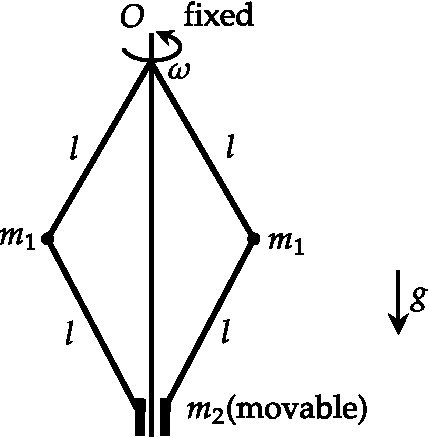
\includegraphics[height=4.5cm,width=4.3cm]{VP-05}
 \end{figure}
\end{exercise}
\begin{answer}$\left. \right. $\\
	 \begin{figure}[H]
		\centering
		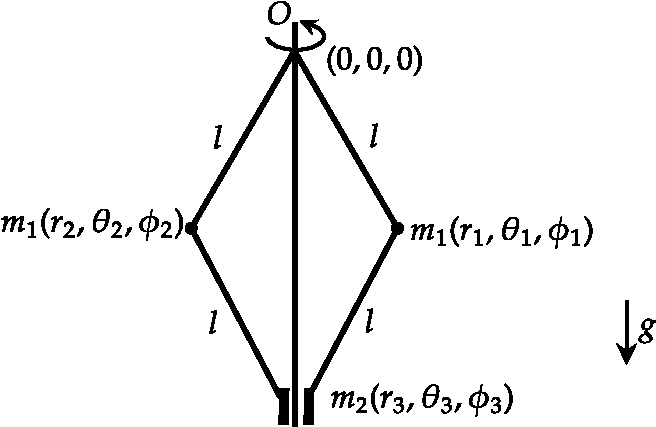
\includegraphics[height=4.5cm,width=6.5cm]{VP-06}
	\end{figure}
	\begin{align*}
\intertext{	(a) Number of Particle,$ N=3$}
	\intertext{The kinetic energy is given by}
	T&=\frac{1}{2} m_{1}\left(\dot{x}_{1}^{2}+\dot{y}_{1}^{2}+\dot{z}_{1}^{2}\right)+\frac{1}{2} m_{2}\left(\dot{x}_{2}^{2}+\dot{y}_{2}^{2}+\dot{z}_{2}^{2}\right)+\frac{1}{2} m_{3}\left(\dot{x}_{3}^{2}+\dot{y}_{3}^{2}+\dot{z}_{3}^{2}\right)
	\intertext{Potential energy assuming $O$ as origin}
	V&=-m_{1} g z_{1}-m_{1} g z_{2}-m_{2} g z_{3}\\
	x_{1}&=r_{1} \sin \theta_{1} \cos \phi_{1}, y_{1}=r_{1} \sin \theta_{1} \sin \phi_{1}, z_{1}=r_{1} \cos \theta_{1}\\
	x_{2}&=r_{2} \sin \theta_{2} \cos \phi_{2}, y_{2}=r_{2} \sin \theta_{2} \sin \phi_{2}, z_{2}=r_{2} \cos \theta_{2}\\
	x_{3}&=r_{3} \sin \theta_{3} \cos \phi_{3}, y_{3}=r_{3} \sin \theta_{3} \sin \phi_{3}, z_{3}=r_{3} \cos \theta_{3}
	\intertext{The kinetic energy in spherical coordinate is given by}
	T&=\frac{1}{2} m_{1}\left(\dot{r}_{1}^{2}+r_{1}^{2} \dot{\theta}_{1}^{2}+r_{1}^{2} \sin ^{2} \theta_{1}^{2} \dot{\phi}_{1}^{2}\right)+\frac{1}{2} m_{2}\left(\dot{r}_{2}^{2}+r_{2}^{2} \dot{\theta}_{2}^{2}+r_{2}^{2} \sin ^{2} \theta_{2}^{2} \dot{\phi}_{2}^{2}\right)\\
	&+\frac{1}{2} m_{3}\left(\dot{r}_{3}^{2}+r_{3}^{2} \dot{\theta}_{3}^{2}+r_{3}^{2} \sin ^{2} \theta_{3}^{2} \dot{\phi}_{3}^{2}\right)\\
	\text{And potential }&\text{energy is given by }V=-m_{1} g r_{1} \cos \theta_{1}-m_{2} g r_{2} \cos \theta_{2}-m_{3} g r_{3} \cos \theta_{3}
	\intertext{Equations of Constraint are -}
	\end{align*}
	(1) Length of mass $m_{1}$ from origin $O$ is fixed, $r_{1}=l$\\
	(2) Length of another mass $m_{2}$ from origin $O$ is fixed, $r_{2}=l$\\
	(3) Both masses $m_{1}$ and $m_{2}$ make same angle with $z$ - axis, $\theta_{1}=\theta_{2}=\theta$\\
	(4) Both masses $m_{1}$ make angle in the $x-y$ plane with $x$ axis as $\phi_{1}=\phi_{2}+c$,\\
	(5) Particle $m_{2}$ makes angle zero with $z$ - axis i.e., $\theta_{3}=0$\\
	(6) Particle $m_{2}$ makes angle zero in $x-y$ plane with $x$ axis i.e., $\phi_{3}=0$,\\
	(7) Particle $m_{2}$ have distance $r_{3}=2 l \cos \theta$ from origin $O$.\\
	So, $K=7$. So degree of freedom (DOF) $=3 N-K=3.3-7=2$
	There is two independent motion (i) linear motion of $m_{2}$ on $z$ axis and (ii) both mass $m_{1}$ rotating about $z$ axis.\\
	So there is a need of two generalized coordinates.\\
	Using equation of constraint one will transform Lagrangian as $L=T-V$
	\begin{align*}
	L&=m_{1} l^{2}\left(\dot{\theta}^{2}+\dot{\phi}^{2} \sin ^{2} \theta\right)+2 m_{2} l^{2} \dot{\theta}^{2} \sin ^{2} \theta+2\left(m_{1}+m_{2}\right) g l \cos \theta\\
\text{	Put the value of }\dot{\phi}&=\omega,\text{ then Lagrangian is given by}\\
	L&=m_{1} l^{2}\left(\dot{\theta}^{2}+\omega^{2} \sin ^{2} \theta\right)+2 m_{2} l^{2} \dot{\theta}^{2} \sin ^{2} \theta+2\left(m_{1}+m_{2}\right) g l \cos \theta\\
	\text{(b) }\left(\frac{\partial L}{\partial \phi}\right)&=0\text{ so $\phi$ is cyclic coordinate hence conjugate momentum}\\ \left(\frac{\partial L}{\partial \dot{\phi}}\right)&=\left(\frac{\partial L}{\partial \omega}\right)=p_{\phi}=2 m_{1} l^{2} \omega \sin ^{2} \theta
	\intertext{is constant during the motion. So, $z$ - component of angular momentum is conserved.}
	\text{(c) }&\frac{d}{d t}\left(\frac{\partial L}{\partial \dot{\theta}}\right)-\frac{\partial L}{\partial \theta}=0\\
	&\left(\frac{\partial L}{\partial \dot{\theta}}\right)=\left(2 m_{1} l^{2} \dot{\theta}+4 m_{2} l^{2} \dot{\theta} \sin ^{2} \theta\right) \\
	&\frac{d}{d t}\left(\frac{\partial L}{\partial \dot{\theta}}\right)=\left(2 m_{1} l^{2}+4 m_{2} l^{2} \sin ^{2} \theta\right) \ddot{\theta}+4 m_{2} l^{2} \sin 2 \theta \dot{\theta}^{2} \\
	&\left(\frac{\partial L}{\partial \theta}\right)=m_{1} l^{2} \omega^{2} 2 \sin \theta \cos \theta+2 m_{2} l^{2} \dot{\theta}^{2} 2 \sin \theta \cos \theta-2\left(m_{1}+m_{2}\right) g l \sin \theta
	\intertext{The equation of motion is given as -}
	\frac{d}{d t}\left(\frac{\partial L}{\partial \dot{\theta}}\right)&-\frac{\partial L}{\partial \theta}=0\\
	\left(2 m_{1} l^{2}+4 m_{2} l^{2} \sin ^{2} \theta\right) \ddot{\theta}&+2 m_{2} l^{2} \sin 2 \theta \dot{\theta}^{2}-m_{1} l^{2} \omega^{2} \sin 2 \theta+2\left(m_{1}+m_{2}\right) g l \sin \theta=0
	\end{align*}
\end{answer}
\section{Aspects of Lagrangian Formulation}
A system with $n$ degrees of freesom possess $x$ equations of motion of the form
$$\frac{d}{dt}\left( \frac{\partial L}{\partial \dot{q}_1}\right)-\frac{\partial L}{\partial q_1}=0 $$
\begin{itemize}
	\item Equations are of second order
	\item motion of the system is determined for all time only when $2n$ initial values are specified
	\item State of the system represented by a point in aa $n$ dimentional configuration space whose coordinaes are 
\end{itemize}